\documentclass{article}
\usepackage{main}

\title{\textbf{Review}\\Tunable Consistency in MongoDB}
\author{Auer Thomas}
\date{\today}

%Read the paper (A copy is in the moodle course):
%William Schultz, Tess Avitabile, and Alyson Cabral. 2019. Tunable consistency in MongoDB.
%Proc. VLDB Endow. 12, 12 (August 2019), 2071–2081.

%Prepare a short summary focusing on the following questions:
% - What kind of transactional guarantees does MongoDB support and how?
% - How do the different options influence performance in distributed and nondistributed settings?


\begin{document}

\maketitle
\horrule{1pt}

\vspace{2em}

The paper ''Tunable Consistency in MongoDB'' reviews consistency trade-offs when using the NoSQL database management system MongoDB. 
The document oriented database provides a variety of consistency levels that the client applications can utilize at operation level.
Many applications may allow infrequent periods of consistency given the high cost of ensuring consistency at all times, at all layers of the DBMS.  
The PACELC theorem, an extension of the CAP theorem, is used as guideline as to what DBMS characteristics are important for the specific use-case of a given environment.

To further provide tunable consistency options, MongoDB implements the parameters for 'WriteConcern' and 'ReadConcern'. 
WriteConcern specifies to which point the data must be commited to the whole, sharded system until the commit-success is passed on to the client. 
As such, the parametrization of ''w:1'' will acknowledge the commit as soon as the write is commited on the primary node that serviced the write, whereas ''w:majority'' will 
require the data to be commited to a majority of all secondary, sharded nodes.\\
ReadConcerns works similarly, in which the data returned must be commited to a certain number of nodes. ''r:1'' will read the data directly from the primary node,
whereas ''r:majority'' requires the data that is requested to be commited on a majority of nodes.\\
With the correct parameter setup, namely ''r:linearizable'' and ''w:majority'', MongoDB is able to provide the strongest consistency guarantees. It is noteworthy that MongoDB users tend to use ''w:1'' and ''r:1'' (as default) based on the importance of latency rather than consistency. Yet the decision to use weaker consistency levels
often works as failures are infrequent and data losses are managable small. 

Since MongoDB allows multiple consistency levels in the same deployment, it is important that this does not impact the performance of the whole system.\\
Writes demand high latency as the data is written to the primary and subsequent secondary nodes. 
Reads are more complex, given the WiredTiger engine in the backend -- Reads are performed with snapshot isolation, meaning that all later updates must be kept in memory.
Time demanding reads, hence, cause memory pressure which must be avoided to limit the impact on transaction performance. 
This is achieved by ''Query Yielding'', where the data is locked for regular intervals. After such an interval ends, the transaction aborts and releases the locks.

\begin{figure}[H]
    \centering
    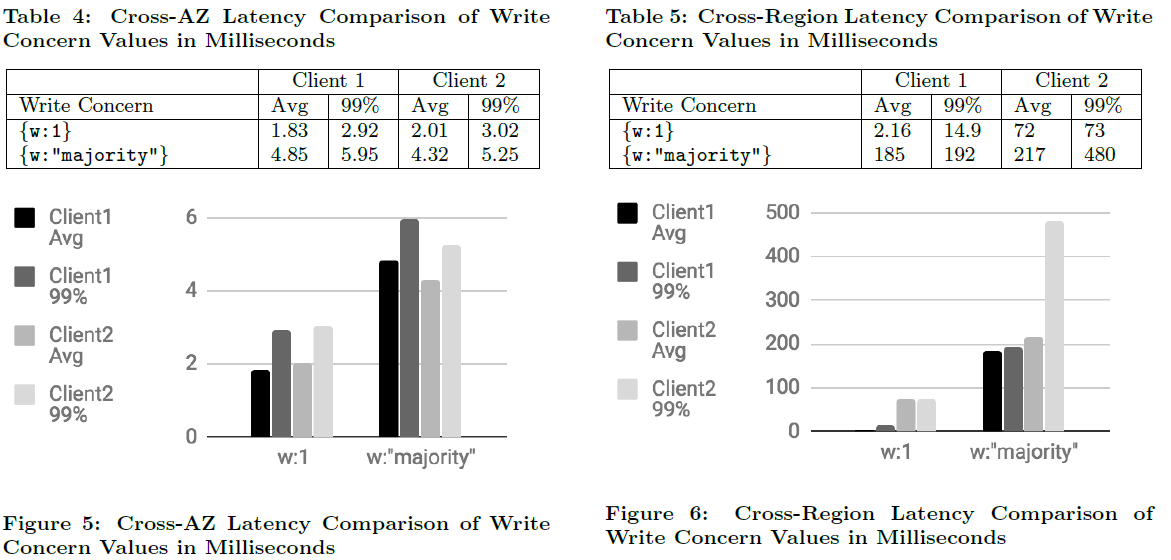
\includegraphics[width=0.9\textwidth]{Tables.png}
\end{figure}




\end{document}